\chapter{Microcontroller Considerations} \label{App:MicrocontrollerConsiderations}
This appendix shows the considerations regarding the used microcontroller, with regards to jitter and speed.

The microcontroller in the project will be an STM32F446RE\cite{ST_STM32F446RE} embedded on an ST NUCLEO-F446RE\cite{ST_NUCLEOF446RE} development board. Code listing \refq{lst:App_A_ToggleCode} was used to test how quickly a pin can be toggled to produce a clock input for the Sample Control (FPGA) module by manipulating the GPIO control registers directly. The microcontroller is running at it's maximum clock frequency of \SIQ{180}{\mega\hertz}. The 

\lstinputlisting[language=C ,style = c,firstnumber=1, linerange=2-8, caption={Code for setting and clearing the CLK pin.}, label={lst:App_A_ToggleCode}]{Appendix/Code/F446REComputeSpeed.tex}

The code will clear the output pin by setting the corresponding pin in the upper 16-bits of the BSRR register in line 4. It will set the pin by setting the corresponding bit in the lower 16-bits of the BSRR register in line 6. The execution time of this code has been measured with an oscilloscope as shown on figure \refq{fig:App_A_SetResetSpeed}.

\begin{figure}[H]
    \centering
    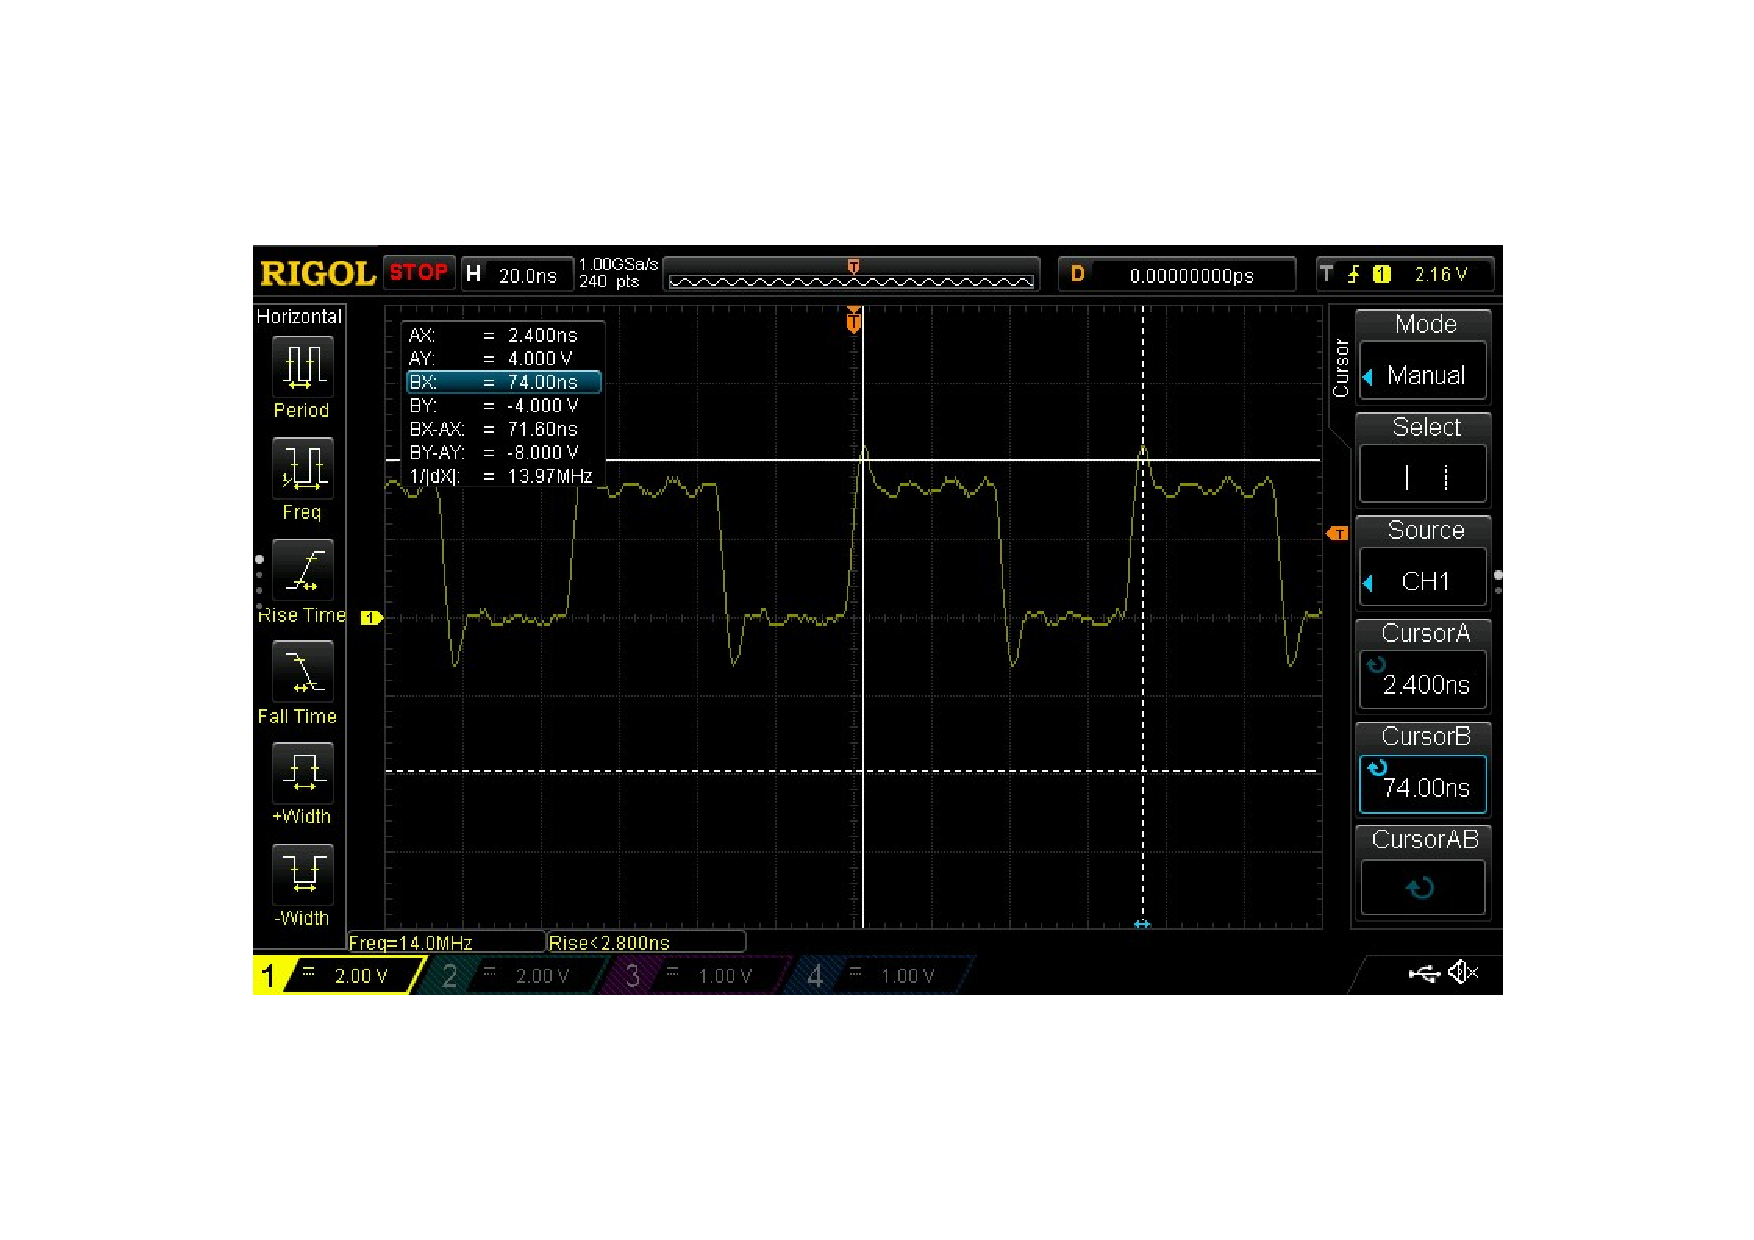
\includegraphics[clip, trim=0 100 0 100, width=1\textwidth]{Appendix/Figures/IOSetResetSpeed.pdf}
    \caption{The CLK pin is toggled by the code in listing \refq{lst:App_A_ToggleCode}. The pulse width is the execution time of the code. There is some ringing present on the signal, this is due to a long probe GND lead.}
    \label{fig:App_A_SetResetSpeed}
\end{figure}

The period of the CLK signal shown on figure \refq{fig:App_A_SetResetSpeed} is \SIQ{71.6}{\nano\second}. It has a 50\% duty cycle so the pulse width, and thus execution time, is \SIQ{35.8}{\nano\second} for toggling the pin by setting and clearing a register. This also means that it takes \SIQ{17.9}{\nano\second} to set 1 register.

It was also tested how much time it takes to change the mode of a GPIO pin. I.e. it was tested how long it takes to switch a pin from being an input to being an output. This will be necessary for the microcontroller to communicate with the FPGA. The code for this can be seen in listing \refq{lst:App_A_SwitchGPIOModes}. Lines 6-7 sets the input mode and turns off pull-up resistors. Lines 9-15 sets the GPIO pin to an output and sets the output to a push-pull type with no pull ups and a maximum slew rate. Lines 4 and 17 will toggle the pin.

\lstinputlisting[language=C ,style = c,firstnumber=1, linerange=10-30, caption={Code for testing the time it takes to swap GPIO pin mode.}, label={lst:App_A_SwitchGPIOModes}]{Appendix/Code/F446REComputeSpeed.tex}

The results for this test can be seen on the oscilloscope snapshot on figure \refq{fig:App_A_OutputInputSpeed}.
\begin{figure}[H]
    \centering
    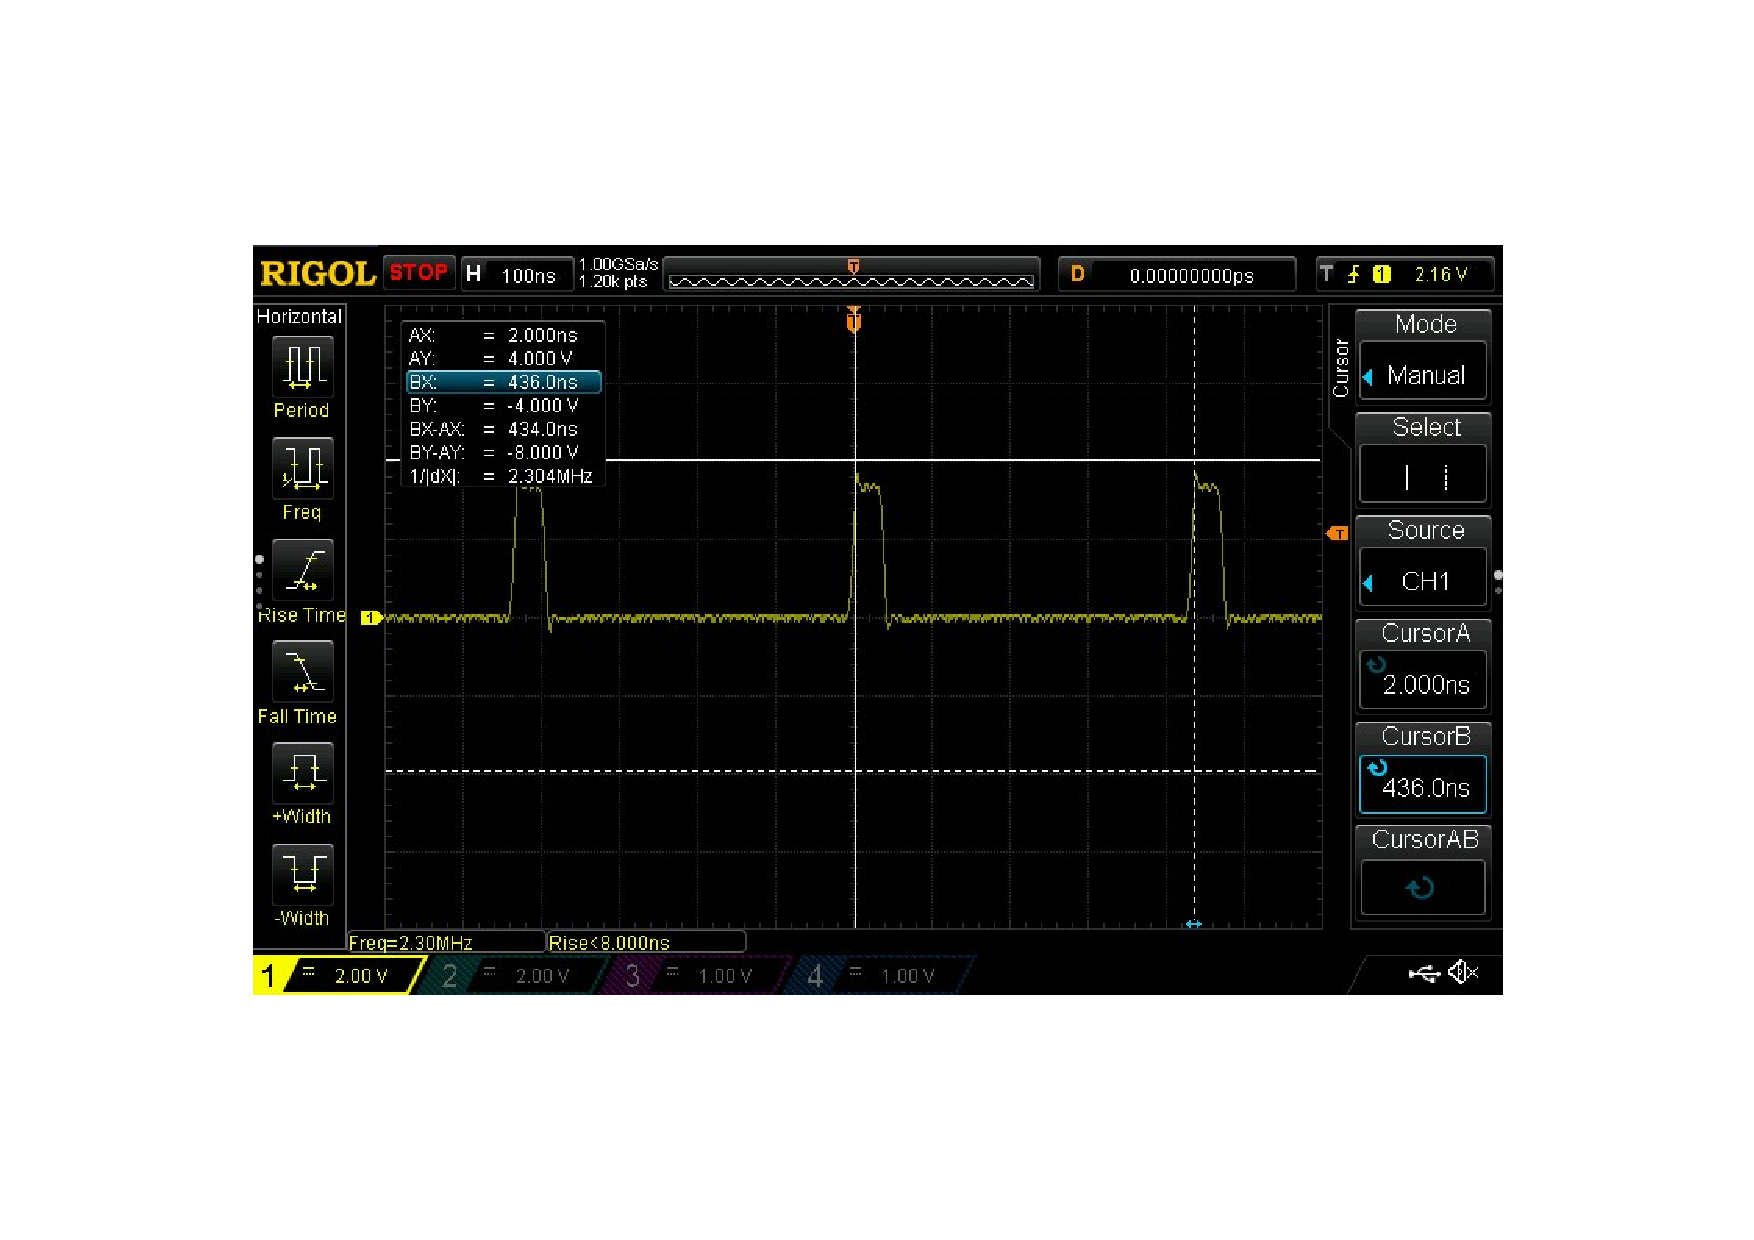
\includegraphics[clip, trim=0 100 0 100, width=1\textwidth]{Appendix/Figures/IOOutputToInputSpeed.pdf}
    \caption{The pin is cleared and changed to input, then back to output and the pin is set with the code in listing \refq{lst:App_A_ToggleCode}.}
    \label{fig:App_A_OutputInputSpeed}
\end{figure}

The period of the toggle pin is \SIQ{434}{\nano\second} as shown in the 3rd quadrant of the snapshot. This means it takes \SIQ{434}{\nano\second} to clear the pin, toggle GPIO modes and set the pin. Previously it was shown that it takes \SIQ{35.8}{\nano\second} to toggle the pin itself, so it takes \SIQ{181.2}{\nano\second} to switch GPIO modes as shown in eq \refq{eq:App_A_ModeSwitch}.

\begin{equation}\label{eq:App_A_ModeSwitch}
    t_{mode} = \frac{t_{total}}{2} - t_{toggle} = \frac{434e-9}{2} - 35.8e-9 = 181.2e-9 
\end{equation}

The CLK pin will be used to CLK data in and out of the Sample Control module, so the rise time of the pin was verified when the pin was set to it's maximum slew rate setting. This can be seen on figure \refq{fig:App_A_RiseTime}.

\begin{figure}[H]
    \centering
    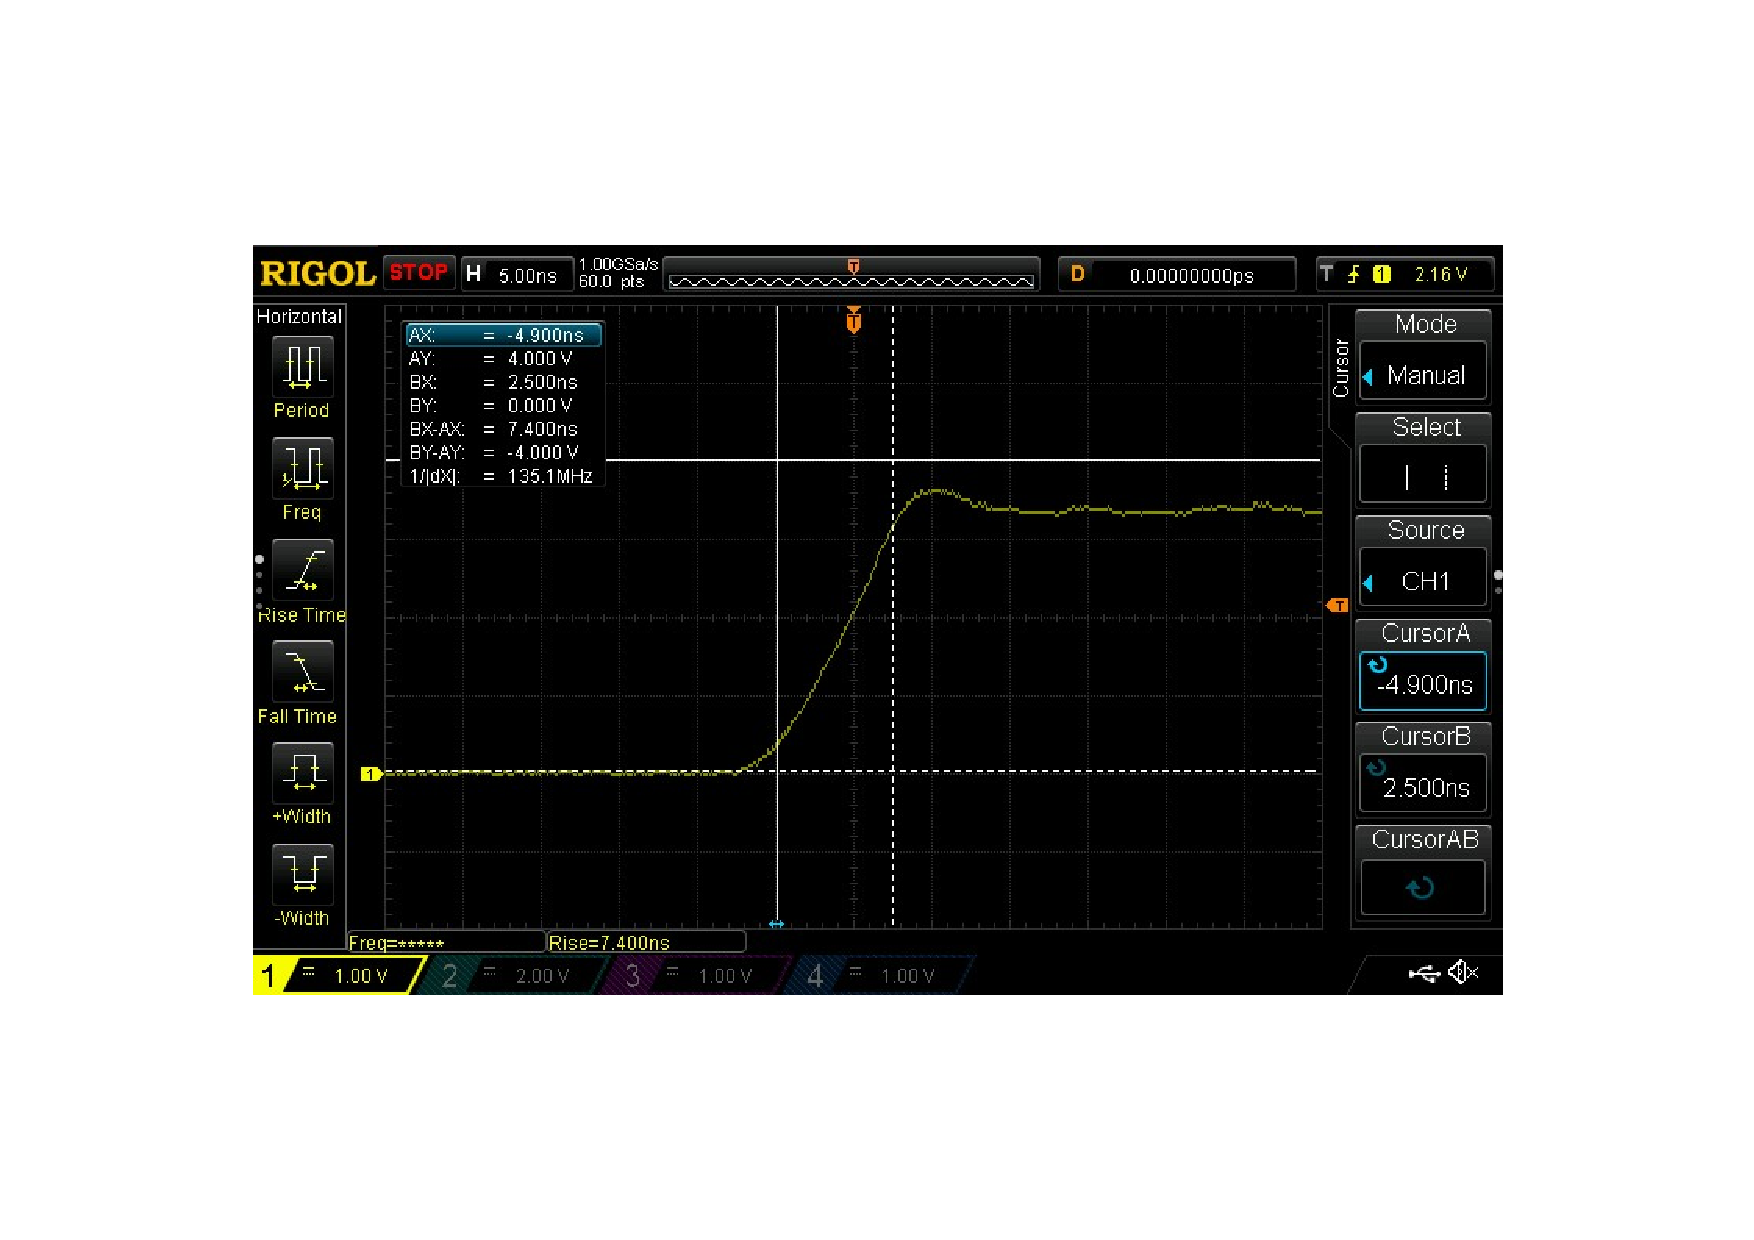
\includegraphics[clip, trim=0 100 0 100, width=1\textwidth]{Appendix/Figures/IORiseFallTime.pdf}
    \caption{The CLK pin is toggled so the rise time can be measured.}
    \label{fig:App_A_RiseTime}
\end{figure}

The rise time of an I/O pin on the microcontroller when the pin is configured to it's maximum slew rate is \SIQ{7.4}{\nano\second} as seen on the oscilloscope snapshot. 

It was considered to use the STM32F446 for controlling the sampling of the ADC's and DAC's directly and for this application it is critical that the acquisition trigger signals for the two ADC's happen at the exact same time with the same period. The jitter of the microprocessor has been measured by toggling an IO pin as can be seen on figure \refq{fig:App_A_Jitter}.

\begin{figure}[H]
    \centering
    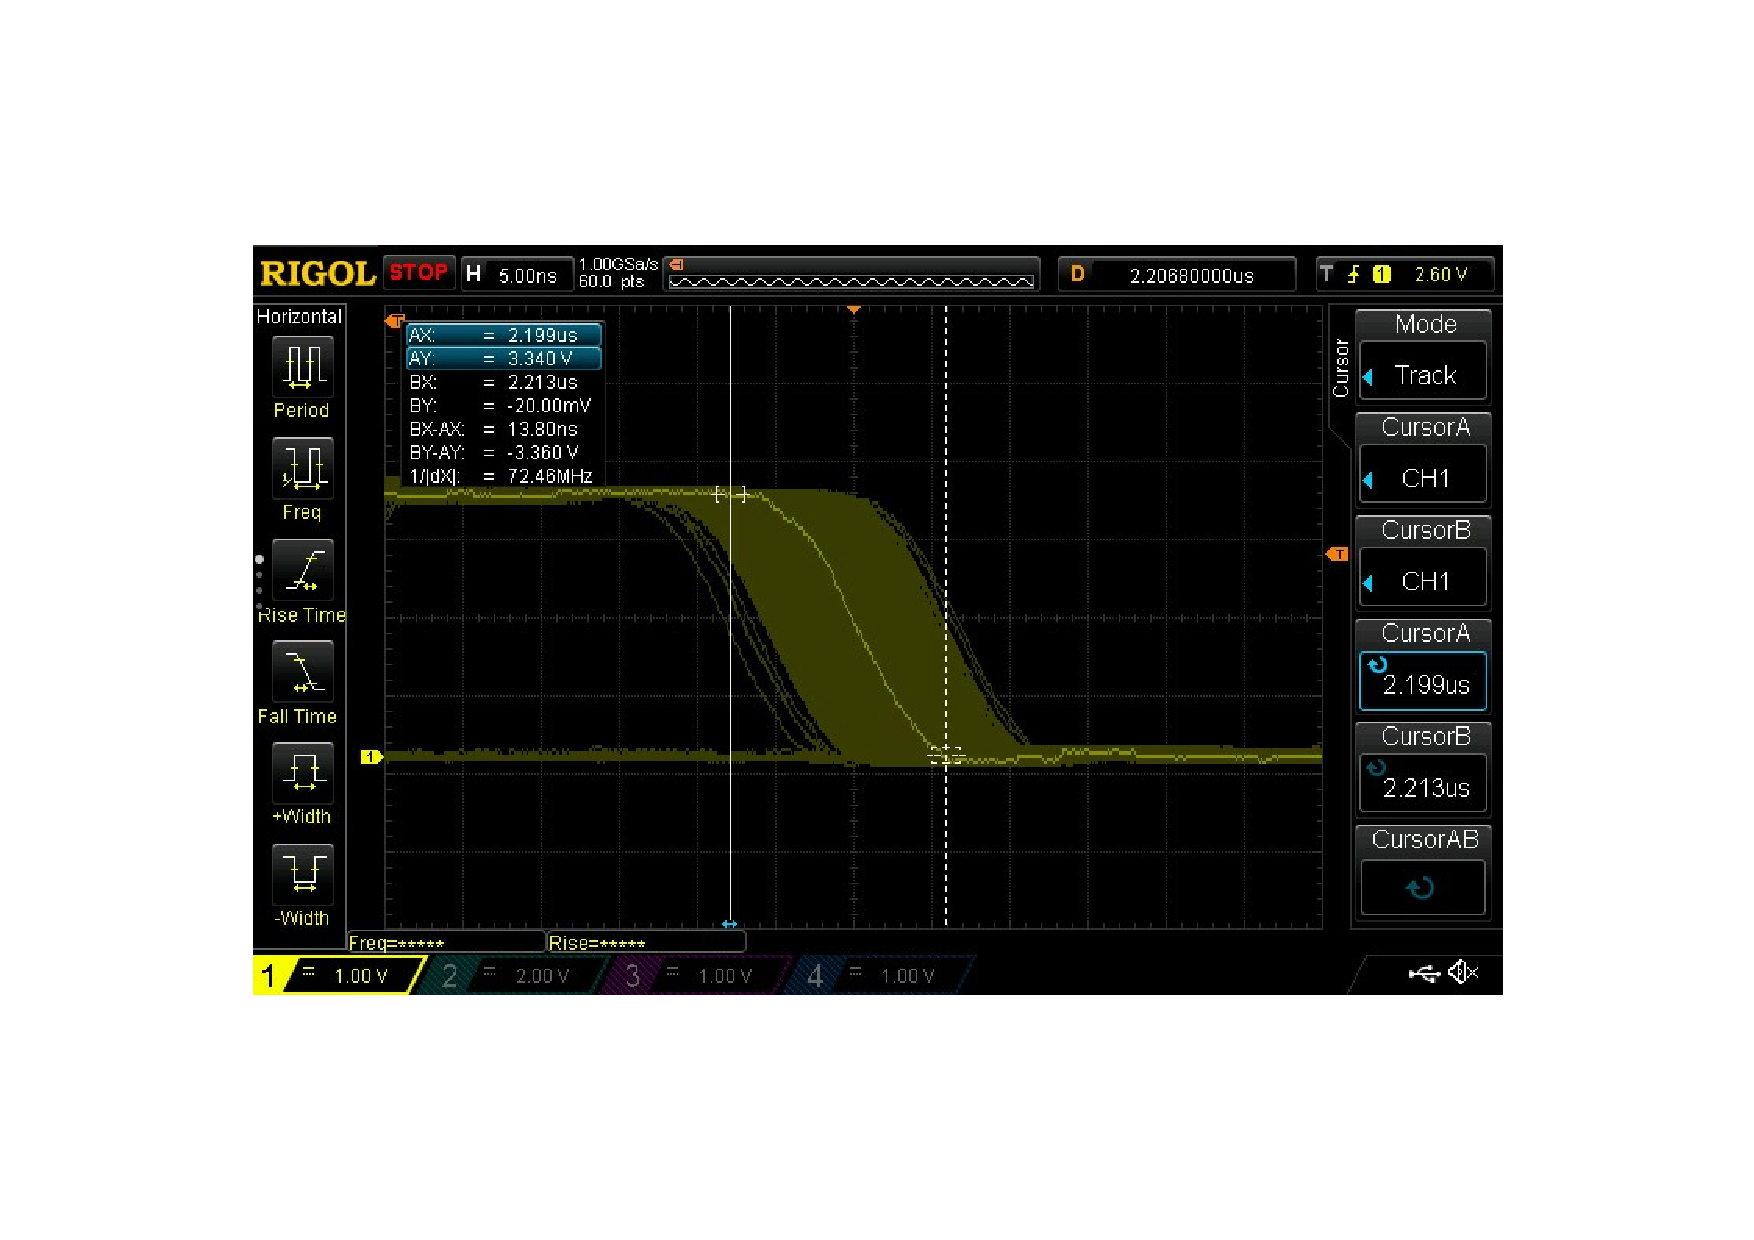
\includegraphics[clip, trim=0 100 0 100, width=1\textwidth]{Appendix/Figures/STM32F446JITTER.pdf}
    \caption{The CLK pin is toggled and the jitter is measured by turning on oscilloscope persistence.}
    \label{fig:App_A_Jitter}
\end{figure}

The STM32F446 has jitter of about \SIQ{13.8}{\nano\second}. This jitter is affected primarily by the PLL circuit that the microprocessors is using to generate the \SIQ{180}{\mega\hertz} core clock frequency from a \SIQ{12}{\mega\hertz} external crystal oscillator. The jitter will get worse depending on how long a time span the sampling is happening over. This jitter will produce a phase error of about 5 degrees at \SIQ{1}{\mega\hertz}. This is because the phase resolution at \SIQ{1}{\mega\hertz} is $\phi_{res} = \frac{360}{1e-6} = 36e6$ degrees per second and with a jitter of \SIQ{13.8}{\nano\second} the jitter will cause a phase error of $\phi_{error} = \phi_{res} \cdot t_{jitter} = 36e6 \cdot 13.8e-9 = 4.986$ degrees at \SIQ{1}{\mega\hertz}. 